% !TEX root = ../lectures_olympics.tex

\chapter{微元法}

	微元法是分析、解决物理问题中的常用方法,也是从部分到整体的思维方法。用该方法可以使一些复杂的物理过程用我们熟悉的物理规律迅速地加以解决,使所求的问题简单化。在使用微元法处理问题时,需将其分解为众多微小的“元过程”,而且每个“元过程”所遵循的规律是相同的,这样,我们只需分析这些“元过程”,然后再将“元过程”进行必要的数学方法或物理思想处理,进而使问题求解。使用此方法会加强我们对已知规律的再思考,从而引起巩固知识、加深认识和提高能力的作用。
微元法解决物理问题的一般思维与操作程序为:
	
	1.决定是否适用微元法。

	2.选择适当的微元。

	3.对微元作物理及数学处理以求结论。
\section{小量分析}

选取一段微元作小量分析是解竞赛题的基本能力之一。如:对于连续体问题(求一个对称物体内部结构之间的联系),需对整体作均匀细分,取出其中的一个微元作“隔离体”加以研究。

\begin{example}
	一质量为$M$、均匀分布的圆环,其半径为$r$,几何轴与水平面垂直,若它能经受的最大张力为$T$,求此圆环可以绕几何轴旋转的最大角速度。
\begin{flushright}
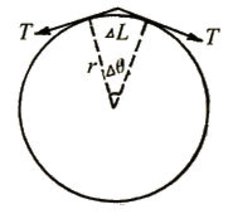
\includegraphics[width = 0.3\textwidth]{images/smallAna-1.pdf} 
\end{flushright}
\tagged{student}{\vspace*{4cm}}
\begin{taggedblock}{teacher}

解析:
\end{taggedblock}
\end{example}

\begin{example}
	半径为R的光滑球固定在水平桌面上,有一质量为$M$的圆环状均匀弹性绳圈,原长为$\pi R$ ,且弹性绳圈的劲度系数为$k$ ,将弹性绳圈从球的正上方轻放到球上,使弹性绳圈水平停留在平衡位置上,如图所示,若平衡时弹性绳圈长为$\pi R$ ,求弹性绳圈的劲度系数$k$。
\begin{flushright}
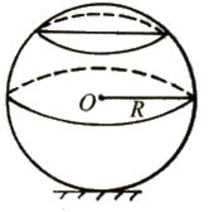
\includegraphics[width = 0.3\textwidth]{images/smallAna-2.pdf} 
\end{flushright}
\tagged{student}{\vspace*{4cm}}
\begin{taggedblock}{teacher}

解析:
\end{taggedblock}
\end{example}

\begin{example}
	粗细均匀质量分布也均匀的半径为分别为$R$和$r$的两圆环相切。若在切点放一质点$m$ ,恰使两边圆环对$m$的万有引力的合力为零,则大小圆环的线密度必须满足什么条件?
\tagged{student}{\vspace*{4cm}}
\begin{taggedblock}{teacher}

解析:$\frac{\rho_1}{\rho_2}=\frac{R}{r}$
\end{taggedblock}
\end{example}


	对于暂态问题,即问题所述情景属于变化全景中的某特殊场景。这时,需截取一与该状态逼近的相邻状态,从而获得一元过程,对该微元过程运用相应得物理规律以求解答。

\begin{example}
	把一个容器内的空气抽出一些,压强降为$p$,容器上有一小孔,上有塞子,现把塞子拔掉,如图所示。问空气最初以多大初速度冲进容器?(外界空气压强为$p_0$ 、密度为$\rho$)
\begin{flushright}
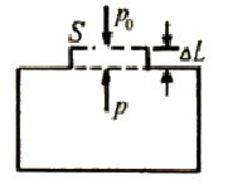
\includegraphics[width = 0.3\textwidth]{images/smallAna-3.pdf} 
\end{flushright}
\tagged{student}{\vspace*{4cm}}
\begin{taggedblock}{teacher}

解析:该题由于不知开始时进入容器内分有多少,不知它们在容器外如何分布,也不知空气分子进入容器后压强如何变化,使我们难以找到解题途径。注意到题目中“最初”二字,可以这样考虑:设小孔的面积为S ,取开始时位于小孔外一薄层气体为研究对象,令薄层厚度为$\Delta L$ ,因$\Delta L$ 很小,所以其质量$\Delta m$ 进入容器过程中,不改变容器压强,故此薄层所受外力是恒力,该问题就可以解决了。
由以上分析,得:\[F = (p_0-p)S\]            
对进入的$\Delta m$气体,由动能定理得:\[F \Delta L = \Delta mv^2\]     
而 \[\Delta m = \rho S\Delta L\]                                     
\\最初中进容器的空气速度$v=\sqrt{\frac{2(p_0-p)}{\rho}}$
\end{taggedblock}
\end{example}


\section{虚功原理}
\begin{description}
\item[虚位移]
质点或质点系在给定瞬时约束系统许可的微小位移。
\item[虚功]
力在虚位移上所做的元功。记为:$\delta W=\vec{F}\cdot\delta\vec{r}$
\item[虚功原理]
质点或质点系在平衡状态下,所有力在任何虚位移上的虚功之和为0.

\begin{equation}
\sum_{i=1}^{N}\vec{F}\cdot\delta\vec{r}=0
\end{equation}


	注意:虚功原理的应用条件是:力系应当满足平衡条件———力系是平衡的
\end{description}

\begin{example}
	如图,一个半径为R的四分之一光滑圆柱面固定在水平桌面上,柱面上有一条单位长度质量为$\rho$的均匀铁链。铁链因A端收到水平拉力F的作用而平衡,B刚好与桌面接触,求水平拉力F的大小。
\begin{flushright}
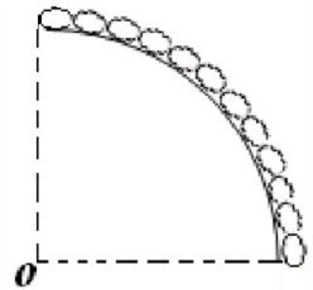
\includegraphics[width = 0.3\textwidth]{images/smallAna-4.pdf} 
\end{flushright}

\tagged{student}{\vspace*{4cm}}
\begin{taggedblock}{teacher}

解析:$F=\rho gR$
\end{taggedblock}
\end{example}


\begin{example}
	如图所示,5根长度均为$l$的质量均为$m$的均质杆,将它们端点铰接成为正六边形机构,固定在天花板上,使六边形在竖直平面内,并用不可伸长的轻绳一端连在下杆中点挂在天花板上,轻绳竖直,求绳上的张力。
\begin{flushright}
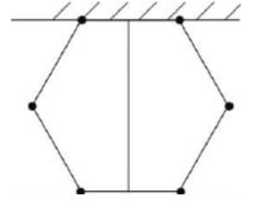
\includegraphics[width = 0.3\textwidth]{images/smallAna-5.pdf} 
\end{flushright}
\tagged{student}{\vspace*{4cm}}
\begin{taggedblock}{teacher}
解析:
\end{taggedblock}
\end{example}


\begin{example}
	如图所示,质量为m、长度为l的均匀柔软粗绳,穿过半径R的滑轮,绳的两端吊在天花板的两个钉子上,两钩间距离为2R,滑轮轴上挂一重物,重物与滑轮总质量为M,且相互间无摩擦,求绳上最低点C处的张力。
\begin{flushright}
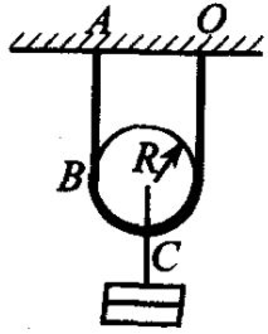
\includegraphics[width = 0.3\textwidth]{images/smallAna-7.pdf} 
\end{flushright}
\tagged{student}{\vspace*{4cm}}
\begin{taggedblock}{teacher}

解析:$T=\frac{M}{2}g+\frac{(\pi-2)R*m}{2l}g$
\end{taggedblock}
\end{example}


\begin{example}
	如图所示,一轻三足支架每边长度均为l,每边与竖直线成同一角度$\theta$,三足置于一光滑水平面上,且恒成一正三角形,现用一绳圈套在三足支架的三足上,使其不能改变与竖直线间的夹角,设三足支架负重为G,试求绳中张力$F_T$。

\begin{flushright}
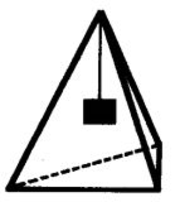
\includegraphics[width = 0.3\textwidth]{images/smallAna-8.pdf} 
\end{flushright}
\tagged{student}{\vspace*{4cm}}
\begin{taggedblock}{teacher}

解析:$F_T=\frac{G\tan\theta}{3\sqrt{3}}$
\end{taggedblock}
\end{example}

\begin{example}
	如图所示,一个外半径为$R_1$,内半径为$R_2$的圆柱形电容器,竖直地插进相对介电常数为$\epsilon_r$的密度为$\rho$的电解液中,若将电容器接上电压为$U$的电源,求电解液中液面上升的高度

\begin{flushright}
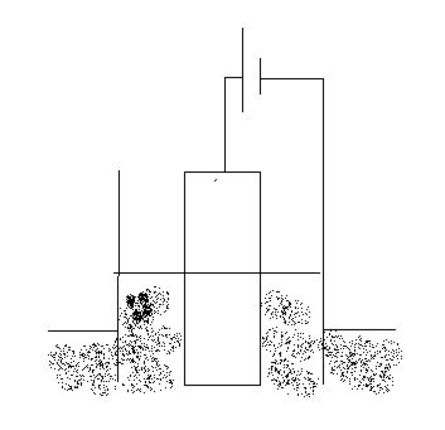
\includegraphics[width = 0.3\textwidth]{images/smallAna-6.pdf} 
\end{flushright}
\tagged{student}{\vspace*{4cm}}
\begin{taggedblock}{teacher}

解析:
\end{taggedblock}
\end{example}



\section{再论微积分}

	对物体进行小量分析后,可能小量并不能在等式中消除,最后要进行求和才能得出最后的答案。于是要联系春季学期学过的积分公式。解此种题需要:寻找合适的变量、列出正确的积分式和好的计算能力。这章着重练习积分式的列出与计算。

\begin{example}
	求一个高度为h,半径为R的圆冠的表面积。
\tagged{student}{\vspace*{4cm}}
\begin{taggedblock}{teacher}
解析:$S=2Rh$,还可趁机复习立体角的概念。
\end{taggedblock}
\end{example}


\begin{example}
	质量均匀为M的细线弯成半径为R的半圆周,试求其对置于圆心的质量为m的质点的万有引力。

\begin{flushright}
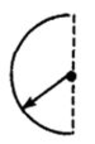
\includegraphics[width = 0.1\textwidth]{images/smallAna-9.pdf} 
\end{flushright}
\tagged{student}{\vspace*{4cm}}
\begin{taggedblock}{teacher}
解析:
\end{taggedblock}
\end{example}

\begin{example}
	真空中电荷Q分布在半径为R的球体内。导出与这一电荷分布相联系的总电能表达式

\tagged{student}{\vspace*{4cm}}
\begin{taggedblock}{teacher}
解析:$E=\frac{3Q^2}{20\pi \varepsilon_0 R}$
\end{taggedblock}
\end{example}

\begin{example}
	匀质椭圆板的半长轴为a,半短轴为b,质量为m。求此椭圆板绕过中心且垂直于椭圆平面轴的转动惯量J。

\tagged{student}{\vspace*{4cm}}
\begin{taggedblock}{teacher}
解析:应用一次垂直轴定理。分别求出绕长轴转动的转动惯量,与绕短轴转动的转动惯量,最后相加。
\end{taggedblock}
\end{example}


\begin{example}
	在x轴下方、$x\>0$区域内是折射率随$y$变化的介质。光线在介质内部沿抛物线$y=ax^2$传播,试求介质折射率$n$关于$y$的函数形式。(已知$y=0$时,介质的折射率为$n_0$)

\begin{flushright}
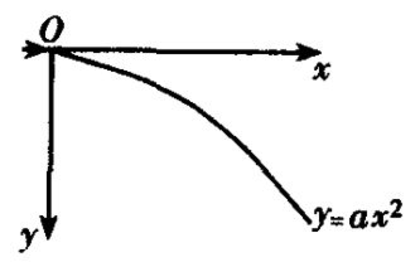
\includegraphics[width = 0.3\textwidth]{images/smallAna-14.pdf} 
\end{flushright}
\tagged{student}{\vspace*{4cm}}
\begin{taggedblock}{teacher}

解析:
\end{taggedblock}
\end{example}


\begin{example}
	一热机工作于两个相同材料的物体A和B之间,两物体的温度分别为$T_A$和$T_B(T_A>T_B)$,每个物体的质量为m、比热恒定均为s。设两个物体的压强保持不变,且不发生相变。
	
	1.假定热机能从系统获得理论上允许的最大机械能,求出两物体A和B最终达到的温度$T_0$的表达式,给出题解的全部过程。
	
	2.由此得出允许获得的最大功的表达式。

\tagged{student}{\vspace*{4cm}}
\begin{taggedblock}{teacher}
解析:
\end{taggedblock}
\end{example}


\begin{example}
	试用毕奥萨伐尔定律求解:一个宽为b、无限长薄铜片,通有电流$I_0$。求铜片中心线正上方$h(h\ll b)$处的P点的磁感应强度。
\tagged{student}{\vspace*{4cm}}
\begin{taggedblock}{teacher}
解析:$B=\frac{\mu_0 I}{2b}$
\end{taggedblock}
\end{example}

\begin{example}
	冬季湖面上的冰经两天的时间,厚度从20mm增为40mm,在此期间冰层底部与顶部的平均温差为8.0K。设冰的密度为$920kg/m^3$,冰的溶解热为$3.20\cdot10^5J/kg$ ,试估算冰的热导率K。
\tagged{student}{\vspace*{4cm}}
\begin{taggedblock}{teacher}
解析:$K=\frac{L\rho (h^2-h_0^2)}{2t*\Delta T}=0.13W/(m*K)$
\end{taggedblock}
\end{example}

\begin{example}
	(整体)热容量分别为$C_1$和$C_2$的两个金属块用一根热容量可忽略不计的粗棍连接起来,整个系统与外界绝热。设t=0时,两金属块的温度分别为$\tau_{10}$和$\tau_{20}$,设单位时间两金属块之间通过粗棍传递的热量正比于两金属块的温度差,比例系数$\alpha$为常量,过程中每一金属块内部各处的温度差可略。试求两金属块温差降为初始温差之半所需的时间$t_0$,以及在$t_0$时刻两金属块各自的温度$\tau_1$和$\tau_2$。
\tagged{student}{\vspace*{4cm}}
\begin{taggedblock}{teacher}
解析:$\tau_1=\frac{2C_1\tau_{10}+C_2(\tau_{10}+\tau_{20})}{2(C_1+C_2)}$

$\tau_2=\frac{2C_2\tau_{20}+C_2(\tau_{20}+\tau_{10})}{2(C_2+C_1)}$
\end{taggedblock}
\end{example}
%%%%%%%%%%%%%%



